\chapter{不稳定性在激光离子加速中的应用}
\label{chap:instability}



\section{常见不稳定性}
等离子体本身是一个复杂的系统,稳定性的研究是其很重要的方向。简单的模型来描述稳定性,正如\ref{fig:stable}所示。假设,存在微小的扰动使得系统偏离平衡状态,稳态系统中,系统通过负反馈及时地平衡扰动,使得系统回复到平衡状态;而对于非稳定系统,  而这种偏离对于非平衡产生正反馈从而加剧了不平衡的程度,使之增长,并最终形成 一种明显效应离开平衡态。
\begin{figure}[!htbp]
  \centering
  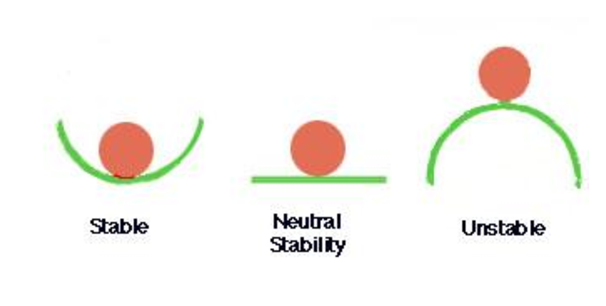
\includegraphics[width=\MyFactor\textwidth]{Img/stable.eps}
  \caption{平衡状态}
  \label{fig:stable}
\end{figure}



 不稳定的形成和增长对于研究激光在等离子体中的吸收,能量沉积,以及热电子的传输等,都有很重要的意义,在快点火聚变\cite{tabak1994ignition},天体物理中有广泛的应用,同时在离子加速中也有重要的影响。等离子体中存在不计其数不稳定性,我们侧重于激光与质密厚靶($\mu m$以上)作用过程中不稳定性的研究。由于激光无法穿透等离子体并在其中传播,因此激光传输过程中的不稳定性就不需要考虑,而激光在等离子体前表面产生的电流向后传播的过程中,存在非常多的不稳定性。
其中常见的流布稳定性包括的有: 韦伯不稳定性\cite{weibel1959spontaneously},双流不稳定性等。韦伯不稳定性,发生在均匀或者近均匀等离子体中。由于电子在动量空间中各向异性分布,通常可以简化理解为不同方向上的两种温度。在微小的磁场扰动下,不同温度的电子产生不同的偏移而产生电流,而这种电流会产生磁场进一步增强原磁场,促进这种扰动并导致不稳定性的增长,最终出现明显的不稳定性的现象。双流不稳定性,是等离子体中常见的现象。当高能粒子束流在等离子体中传播时,电子和离子束流具有不同的速度,而这种不同速度分布会激发等离子体波以及不稳定性。如图\ref{fig:twoStream},当高能电子束流入射到等离子体中,其速度分布出现一个局部的凸起。如果一种等离子体波的相速度处于如图所示的位置,则大于相速度的‘快电子’数目要多于‘慢电子’,粒子的能量将转化至此等离子体波中。

\begin{figure}[!htbp]
  \centering
  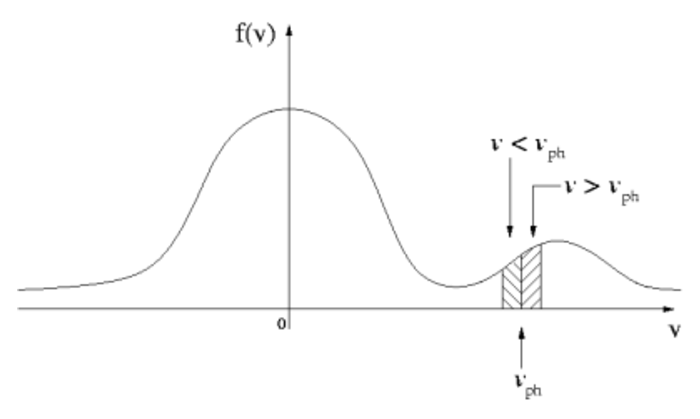
\includegraphics[width=\MyFactor\textwidth]{Img/twoStream.eps}
  \caption{双流不稳定性}
  \label{fig:twoStream}
\end{figure}


当激光与等离子体前表面产生的高能电子正向电流在等离子体中传播时,由于电中性的要求,背景电子存在回流。这种回流与正向电流方向相反,并由此激发与电流的方向垂直的成丝分布,而这一现象和以上三种不稳定性相关。如图\ref{fig:Bret2005}\cite{bret2005characterization},其中成丝不稳定性与韦伯不稳定性属于不稳定性增长方向与扰动方向垂直的横向模式,双流不稳定性属于纵向模式。在非相对论领域,双流不稳定性处于主要的地位;而对于相对论电流,成丝不稳定性占据主导地位。然而在成丝的过程中,各种模式共同存在,并通过偶和的方式决定了不稳定性的增长率等。

\begin{figure}[!htbp]
  \centering
  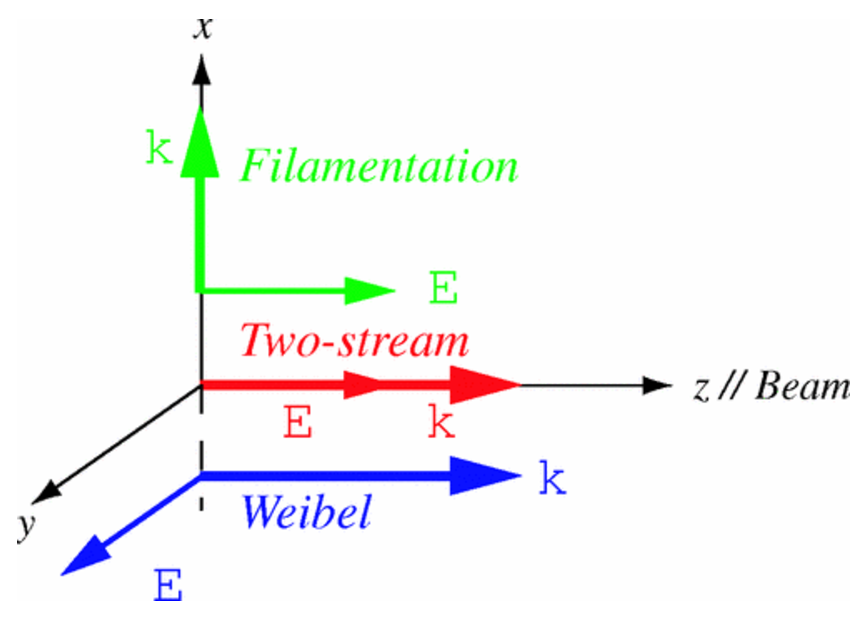
\includegraphics[width=\MyFactor\textwidth]{Img/Bret2005.eps}
  \caption{成丝过程中的不稳定模式}
  \label{fig:Bret2005}
\end{figure}

基于无限空间中高能电子束流在等离子体中的传播模型,A. Bret\cite{bret2005characterization,bret2004collective}研究了三种模式共同存在下,成丝不稳定性的增长率以及成丝具体分布的研究,得出如下结论。
\begin{equation}
\label{eqn:maxGrowth}
{\sigma}_M= \frac{\sqrt{3}}{2^{4/3}}(\frac{\alpha}{{\gamma}_b})^{1/3} {\omega}_p
\end{equation} 
其中${\sigma}_M$是最大增长率,$\alpha=n_b/n_p$,$n_b$是回流的密度,$n_p$是正向电流的密度,${\gamma}_b=1/sqrt{1-{\beta}^2}$,$\beta=V_b/c$,${\omega}_p=(4 \pi n_p e^2/m_e)^{1/2} $是等离子体频率。

\begin{equation}
\label{eqn:filamentSpace}
L_f \approx \pi {\lambda}_s \sqrt{V_{tp}/V_b}
\end{equation} 

其中$L_f$是成丝间隔,$V_{tp}$是前向电流的速度, $V_b$是回流的速度。


然而在激光与有限厚度等离子体作用的过程中,高能电子束流在等离子体中的传播情况出现了变化。由于靶厚有限,回流作用在靶后的位置得到的明显的增强,不稳定性的增长率以及成丝分布发生的变化。由此使得电子的分布受到影响,电子在靶后表面相应的形成的鞘层场也有一定的变化,最终影响了出射离子的分布。


\section{高能电子束流在有限厚度靶中的成丝现象}



电流在等离子体的传播,不稳定性的存在是必然的,其产生需要一定的时间以及距离,可以说,对于厚度在$10\mu m$以上的靶,这种不稳定性的增长有可能变得十分的,然而对于厚度仅在$\mu m$的靶,不稳定性分布在离子加速中是可以不考虑的,因为不稳定性的影响还无法改变离子的能量以及分布的情况。


对于无限厚度的靶,当前表面有超强相对论激光与靶作用电流,由于电中性的要求,一部分电子需要以回流的方式向相反的方向运动,形成相应的回流电流,这种相对运动的电流构成了不稳定性的基础,当相对运行的流的强度达到一定阈值,不稳定性的增长率急剧增长,并迅速建立起不稳定的特征。然而在一般情况下由于回流电子多属于背景热电子,其温度和速度都相应的较低,电子数目比较的多,总体上实现电荷平衡,但是其电流强度很难和前向电流相比,很难真正的使得不稳定急剧的增长。






然而实际中的靶很难使无限的厚度,因此我们考虑在有限厚度的靶中的流不稳定性的情况。因为是有限大小的靶,因此其尺寸就是十分重要的因素之一,因为当电子到达边界的时候,电子的回流的相应就不同于在靶内部的情况。考虑相对论情况下的强电流在有限厚度的靶中的传播,当电流达到靶后表面的时候,一部分电子会以回流的方式反向运动,其速度远大于背景电子的速度,而且相应的电流的强度和前向电流的强度可比拟,因此这种情况下的,相向而行的电流之间形成的硫不稳定性的增长就可以达到很高的增长率。模型很简单如下: 有10$\mu m$厚度的靶,其密度高于临界密度,因此激光脉冲很难穿透靶进入内部,电流的形成主要分布在了前表面,而相应的电流的传播在靶中形成一定影响,背景电子的回流效应完成了电中性的要求,随后当前向电子达到靶后的时候,有相应的反射的想象的出现,而此时的电流的相对增长的趋势就变得很明显了,而且其强度可以比拟。不稳定性的增长率迅速的上升达到一个相应的值。而造成这种现象产生的根源在于电流的发射使得回流电流变得可以满足不稳定性快速增长的要求,而相应的不稳定性的增长率及不稳定现象的描述可以参考流布稳定性的分析的工作。其相应的仿真结果如下:

首先磁场的分布的情况,成丝现象的最基本的特征是在相应的位置处有磁场的生成,在我们可以很清楚的看到磁场的在靶后表面的位置的分布,这说明不稳定性的明显的电流的成丝分布在后表面的位置得到了很强的增长。考虑不稳定性出现的时间,是前向电流达到靶后表面的位置,而正是由于反射的作用的存在,因此回流方向的电流得到了很大程度上的增强,使得不稳定的增长率在很短的时间内得到了急剧的增长。在随后的时间里,反射持续存在并且在相应的位置处产生很明显的不稳定的分布,其中电流的成丝的现象的出现的位置仅仅分布在靶的后表面的位置处。为了探究其不稳定性的产生的源头,后表面电流反射的增强效应,我们对于不同位置处的电子的密度在最强的不稳定性出现的前后进行了相应的跟踪分析切片的处理。得到的结论如下:
1不稳定性的出现首先在于靶的后表面
2 不稳定性的出现的时间在与激光的产生的强电流传播到靶后表面的位置
3 其成丝现象的条纹的间隔随着时间的变化有着一定的增长,和电流的强度有着相应的关系
由此可见这种不稳定性的出现的一个重要的原因就在于靶后表面的反射的作用对于回流的增强。但是否所有的这种后表面的反射都会在很大程度上增强不稳定性的增长。问题在于不稳定的出现的原因在, 对于厚度在微米量级的靶,即便是后表面的反射作用,其回流也无法和前向电流进行比拟,存在数量级上的恶差距,无法满足不稳定性快速增长的条件。而对于厚靶(十微米以上或者更厚),随着前向电流的传播及耗散,达到靶后的时候,强度基本和回流相当,因此不稳定性的增长趋势也就相应的增加了很多。为了验证这一点,我们做了相应的实验,当靶厚低于一定的值之后,这种不稳定性现象不再出现。相反,当靶厚较高时,很容易出现不稳定的想象,而且这些现象十分的稳定。对于高光强还是相对较低的光强,都存在很明显的不稳定性的特征。再次基础上研究了电子产生的后表面加速电场,以及相应的质子的加速的情况。由于成丝的出现,因此电子的分布呈现出一定的周期性的调制结构,相应的加速电场的分布以及质子的分布也有同样的特征。
